\begin{figure*}[!t]
  \centering
  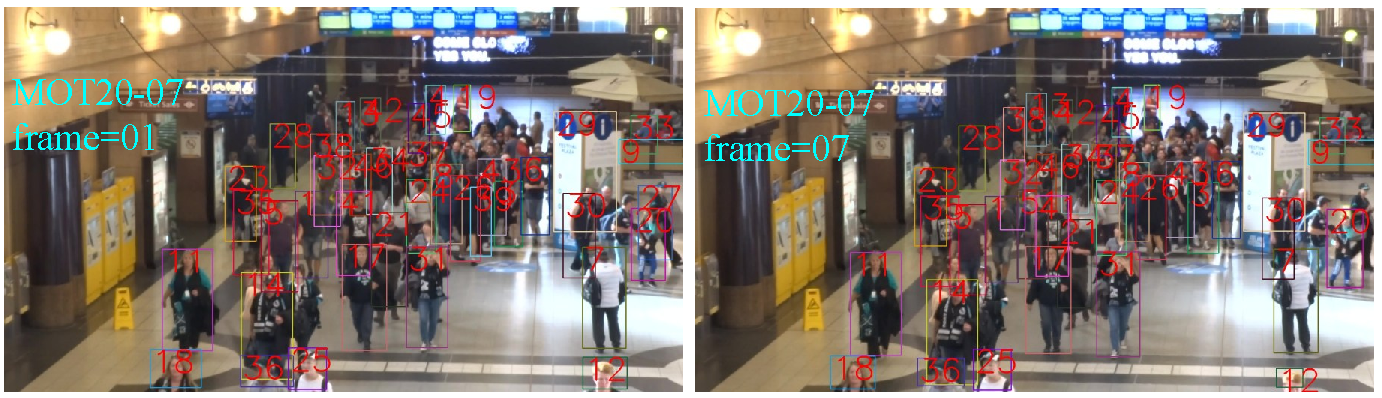
\includegraphics[width=1\textwidth]{imgs/rebuttal/MOT20_v1.pdf}
  %\vskip -2ex
  \caption{Visualizing the tracking performance of the OmniTrack method in dense crowds (MOT20~\cite{dendorfer2020mot20}).}
  \label{fig:MOT20}
  %\vskip -2ex
\end{figure*}

\section{Discussion}
\subsection{Societal Impacts}
The OmniTrack framework is promising to enhance the safety and reliability of autonomous systems by improving Multi-Object Tracking (MOT) in panoramic settings, which is essential for applications such as self-driving cars and robots.
Its ability to process panoramic fields of view while mitigating distortions ensures robust performance in dynamic, real-world environments. 
These advancements have the potential to benefit a wide range of industries, particularly in navigation for individuals with visual impairments, drone-assisted rescue, and hazardous object detection. Furthermore, the development of the QuadTrack dataset, designed for high-speed sensor motion and panoramic field-of-view applications, fills a critical gap in available resources. 
Aim to make both the dataset and the associated code publicly available, we intend to accelerate progress in the field of omnidirectional multi-object tracking,
%
ultimately advancing the safety, efficiency, and inclusivity of automated systems in everyday life. Yet, it is inevitable that the deep model exhibits some false positives and negatives, and its practical deployment must account for the inherent uncertainty of deep neural networks. 
Additionally, while the technology is intended for benign applications, there exists a small risk of misuse, including potential military applications, and it may not be suitable for privacy-sensitive environments.

\subsection{Limitations and Future Work}
Although OmniTrack shows strong potential in the field of panoramic image tracking, it still has some limitations. 
While it does not exhibit ID confusion when targets are severely occluded, track loss can still occur in such scenarios. 
Future work could focus on addressing target occlusion, with one promising solution being multi-sensor fusion, such as integrating point cloud depth information to mitigate occlusion. 
This approach could extend 2D tracking to 3D tracking. Additionally, employing multiple agents that collaborate and share sensor information may enhance tracking performance,  ultimately reducing track loss caused by occlusion and improving overall system robustness.

%
